\documentclass[bachelor, och, labwork]{shiza}
% параметр - тип обучения - одно из значений:
%    spec     - специальность
%    bachelor - бакалавриат (по умолчанию)
%    master   - магистратура
% параметр - форма обучения - одно из значений:
%    och   - очное (по умолчанию)
%    zaoch - заочное
% параметр - тип работы - одно из значений:
%    referat    - реферат
%    coursework - курсовая работа (по умолчанию)
%    diploma    - дипломная работа
%    pract      - отчет по практике
% параметр - включение шрифта
%    times    - включение шрифта Times New Roman (если установлен)
%               по умолчанию выключен
\usepackage{subfigure}
\usepackage{tikz,pgfplots}
\pgfplotsset{compat=1.5}
\usepackage{float}

%\usepackage{titlesec}
\setcounter{secnumdepth}{4}
%\titleformat{\paragraph}
%{\normalfont\normalsize}{\theparagraph}{1em}{}
%\titlespacing*{\paragraph}
%{35.5pt}{3.25ex plus 1ex minus .2ex}{1.5ex plus .2ex}

\titleformat{\paragraph}[block]
{\hspace{1.25cm}\normalfont}
{\theparagraph}{1ex}{}
\titlespacing{\paragraph}
{0cm}{2ex plus 1ex minus .2ex}{.4ex plus.2ex}

% --------------------------------------------------------------------------%


\usepackage[T2A]{fontenc}
\usepackage[utf8]{inputenc}
\usepackage{graphicx}
\graphicspath{ {./images/} }
\usepackage{tempora}

\usepackage[sort,compress]{cite}
\usepackage{amsmath}
\usepackage{amssymb}
\usepackage{amsthm}
\usepackage{fancyvrb}
\usepackage{listings}
\usepackage{listingsutf8}
\usepackage{longtable}
\usepackage{array}
\usepackage[english,russian]{babel}

\usepackage[colorlinks=false]{hyperref}
\usepackage{url}

\usepackage{underscore}
\usepackage{setspace}
\usepackage{indentfirst} 
\usepackage{mathtools}
\usepackage{amsfonts}
\usepackage{enumitem}
\usepackage{tikz}
\usepackage{minted}

\newcommand{\eqdef}{\stackrel {\rm def}{=}}
\newcommand{\specialcell}[2][c]{%
\begin{tabular}[#1]{@{}c@{}}#2\end{tabular}}

\renewcommand\theFancyVerbLine{\small\arabic{FancyVerbLine}}

\newtheorem{lem}{Лемма}

\begin{document}

% Кафедра (в родительном падеже)
\chair{теоретических основ компьютерной безопасности и криптографии}

% Тема работы
\title{Дискретное логарифмирование в конечном поле}

% Курс
\course{5}

% Группа
\group{531}

% Факультет (в родительном падеже) (по умолчанию "факультета КНиИТ")
\department{факультета КНиИТ}

% Специальность/направление код - наименование
%\napravlenie{09.03.04 "--- Программная инженерия}
%\napravlenie{010500 "--- Математическое обеспечение и администрирование информационных систем}
%\napravlenie{230100 "--- Информатика и вычислительная техника}
%\napravlenie{231000 "--- Программная инженерия}
\napravlenie{100501 "--- Компьютерная безопасность}

% Для студентки. Для работы студента следующая команда не нужна.
% \studenttitle{Студентки}

% Фамилия, имя, отчество в родительном падеже
\author{Улитина Ивана Владимировича}

% Заведующий кафедрой
% \chtitle{} % степень, звание
% \chname{}

%Научный руководитель (для реферата преподаватель проверяющий работу)
\satitle{профессор} %должность, степень, звание
\saname{В. А. Молчанов}

% Руководитель практики от организации (только для практики,
% для остальных типов работ не используется)
% \patitle{к.ф.-м.н.}
% \paname{С.~В.~Миронов}

% Семестр (только для практики, для остальных
% типов работ не используется)
%\term{8}

% Наименование практики (только для практики, для остальных
% типов работ не используется)
%\practtype{преддипломная}

% Продолжительность практики (количество недель) (только для практики,
% для остальных типов работ не используется)
%\duration{4}

% Даты начала и окончания практики (только для практики, для остальных
% типов работ не используется)
%\practStart{30.04.2019}
%\practFinish{27.05.2019}

% Год выполнения отчета
\date{2023}

\maketitle

% Включение нумерации рисунков, формул и таблиц по разделам
% (по умолчанию - нумерация сквозная)
% (допускается оба вида нумерации)
% \secNumbering

%-------------------------------------------------------------------------------------------

\section{Постановка задачи}

    \textbf{Цель работы} - изучение основных методов дискретного
    логарифмирования в конечном поле и их программная реализация. 

    Порядок выполнения работы:
    \begin{enumerate}
        \item Рассмотреть метод Гельфонда-Шенкса вычисления дискретного
        логарифма и привести его программную реализацию;
        \item Рассмотреть $(\rho)$-метод Полларда вычисления дискретного
        логарифма и привести его программную реализацию;
        \item Рассмотреть метод вычисления дискретного логарифма в конечных
        полях;
    \end{enumerate}

\section{Теоретические сведения}

    \subsection{Дискретный логарифма}

        Пусть $G = \langle a \rangle$ "--- конечная циклическая группа порядка
        $m$, т.е. $$G = \{a^0 = 1, a^1 = a, a^2, \dots, a^{m - 1} \}.$$

        \underline{Определение:} Дискретным логарифмом элемента $b \in G$
        называется число $x \in \{0, 1, \dots, m - 1\}$, для которого $$a^x =
        b.$$ Обозначение $x = \log_a b$.

        Задача нахождения дискретного логарифма имеет большую сложность
        вычислений.

        Алгоритм Гельфонда-Шенкса вычисления дискретного логарифма
        осуществляется в произвольной циклической группе, элементы которой
        линейно упорядоченны.

    \subsection{$\rho$-метод Полларда}

        Дана конечная циклическая группа $G = \langle a \rangle$ порядка $m$ и
        элемент $b \in G$. Причем группа разбита на три примерно равные части
        $U_1, U_2, U_3$ с простым алгоритмом проверки вхождения элементов в эти
        части.

        Определяется преобразование $f: G \to G$ для элементов $x \in G$ по
        формуле:

        \[f(x) =
            \begin{cases}
                bx, \text{ если } x \in U_1,\\
                x^2, \text{ если } x \in U_2,\\
                ax, \text{ если } x \in U_3.
            \end{cases}
        \]

        Для случайно выбранного значения $s \in Z_m$ рассматривается
        рекуррентная последовательность: $$y_i = f(y_{i - 1}), i \geq 1, y_0 =
        a^s.$$

        Тогда $y_i = a^{\alpha_i} b^{\beta_i}$ для рекуррентно заданных
        последовательностей:

        \[\alpha_0 = s, \text{ } \alpha_{i + 1} = \begin{cases}
            \alpha_i \pmod m, \text{ если } y_i \in U_1,\\    
            2\alpha_i \pmod m, \text{ если } y_i \in U_2,\\    
            \alpha_i + 1 \pmod m, \text{ если } y_i \in U_3;\\    
        \end{cases}
        \]

        \[\beta_0 = 0, \text{ } \beta_{i + 1} = \begin{cases}
            \beta_i + 1 \pmod m, \text{ если } y_i \in U_1,\\    
            2\beta_i \pmod m, \text{ если } y_i \in U_2,\\    
            \beta_i \pmod m, \text{ если } y_i \in U_3.\\    
        \end{cases}
        \]

        Так как при этом $$y_i = a^{\alpha_i} b^{\beta_i} = a^{\alpha_i}
        (a^x)^{\beta_i} = a^{\alpha_i + \beta_i x},$$
        то выполняется $$\log_a y_i = \beta_i x + \alpha_i \pmod m.$$

    \subsection{Индекс-метод дискретного логарифмирования в конечном простом поле}

        Если $h = p_1^{k_1} \dots p_r^{k_r},$ то $\log_a h = k_1 \log_a p_1 +
        \dots + k_r \log_a p_r.$

        Даны $a$ "--- образующий элемент группы $GF(p)^*$ и $h \in GF(p)^*.$
        Требуется найти $x = \log_a h.$ Будем считать, что $GF(p) = Z_p.$ Пусть
        $B$ "--- некоторое натуральное число - параметр метода, который
        определяет факторную базу $S_B = \{2, 3, 5, \dots, q \}$ "--- множество
        первых простых чисел, не превосходящих $B$, $|S_B| = \pi(B)$. Значение
        параметра $B$ выбирается таким образом, чтобы минимизировать сложность
        алгоритма.

        Для всех $1 \leq i \leq \pi(B)$ обозначим $x_i = \log_a q_i \in Z_{p -
        1},$ где $q_i \in S_B.$

        Алгоритм аналогичен субэкспоненциальным алгоритмам факторизации, но
        соответствующие алгоритмы дискретного логарифмирования обладают одной
        особенностью – эти алгоритмы условно можно разделить на два этапа:

        \begin{enumerate}
            \item сначала по заданному $p$ надо выбрать факторную базу и
            определить логарифмы элементов факторной базы (при фиксированном $p$
            этот этап надо проделать только один раз);
            \item на втором этапе с использованием известных логарифмов
            элементов факторной базы по заданному $h \in Z_p^*$ необходимо найти
            $\log_a h$ (этот этап может производиться неоднократно).
        \end{enumerate}


\section{Результаты работы}

    \subsection{Описание и псевдокод алгоритмов факторизации целых чисел}

        \underline{Алгоритм 1 - Метод Гельфонда-Шенкса}\\
            \textit{Вход}: Конечная линейно упорядоченная группа $G = \langle a
            \rangle$, верхняя оценка порядка группы $|G| \leq B$ и $b \in G$.\\
            \textit{Выход}: $x = \log_a b$.\\
            \underline{Шаг 1.} Вычислить $r = [\sqrt{B}] + 1$. Вычислить
            элементы $a, a^2, \dots, a^{r-1}$ и упорядочить по второй координате
            множество пар $(k, a^k)$, $1 \leq k \leq r - 1$.\\
            \underline{Шаг 2.} Вычислить $a_1 = a^{-r}$. Для каждого $0 \leq i
            \leq r - 1$ вычислить $a_1^i$ и проверить, является ли элемент
            $a_1^i b$ второй координатой какой-нибудь пары из упорядоченного
            множества, построенного на шаге $1$. Если $a_1^i b = a^k$, то
            $a^{-ri} b = a^k, b = a^k a^{ri} = a^{k + ri}$ запомнить $k + ri$.\\
            \underline{Шаг 3.} Найти число $x$, равное наименьшему значению
            среди чисел $k + ri$, вычисленных на предыдущем шаге. В результате
            получаем $x = \log_a b$.\\
            
        \underline{Псевдокод:}
            \begin{minted}[breaklines,fontsize=\small]{text}
                Функция Полларда_Ро(число, эпсилон):
                    Если n == 1:
                        Вернуть 1
                    Если n четное:
                        Вернуть 2
                    
                    Пусть T = вычислить_T_(эпсилон)
                    Пусть rng - генератор случайных чисел
                    Пусть x = случайное_Число_Из_Диапазона(2..n)
                    Пусть y = x
                    Пусть d = 1
                    
                    Функция f(x):
                        Вернуть (x * x + 1) % n
                    
                    Пока d == 1 и количество_повторений < T:
                        x = f(x)
                        y = f(f(y))
                        Если x > y:
                            d = НОД(x - y, n)
                        Иначе:
                            d = НОД(y - x, n)
                        T = T - 1
                    
                    Вернуть d       
            \end{minted}

            Трудоемкость алгоритма $O(\sqrt{B} \log B)$.\\

        \underline{Алгоритм 2 - $\rho$-метод Полларда вычисления дискретного
        логарифма}\\
        \underline{в прооизвольной циклической группе}\\
            \textit{Вход}: конечная группа $G = \langle a \rangle$ порядка $m$,
            элемент $b \in G$, определенная выше функция $f: G \to G$ и число
            $\varepsilon > 0$.\\
            \textit{Выход}: $x = \log_a b$ с вероятностью не менее $1 -
            \varepsilon$.\\
            \underline{Шаг 1.} Вычислить $k = [\sqrt{2\sqrt{m}\ln
            \frac{1}{\varepsilon}}] + 1$.\\
            \underline{Шаг 2.} Положить $i = 1$, выбрать случайное значение $s
            \in Z_m$ и вычислить $y_0 = a^s, y_1 = f(y_0)$. Запомнить две тройки
            $(y_0, \alpha_0, \beta_0), (y_1, \alpha_1, \beta_1)$ и перейти к
            шагу $3$.\\
            \underline{Шаг 3.} Положить $i = i + 1$, вычислить $y_i =
            f(y_{i-1}), y_{2i} = f(f(y_{2i - 2})),$ запомнить две тройки $(y_i,
            \alpha_i, \beta_i), (y_{2i}, \alpha_{2i}, \beta_{2i})$ и перейти к
            шагу $4$.\\
            \underline{Шаг 4.} Если $y_i \neq y_{2i}$, то проверить условие $i <
            k$. Если это условие выполнено, то перейти к шагу $3$. Иначе
            закончить вычисления и сообщить, что значение $x = \log_a b$
            вычислить не удалось. Если же $y_i = y_{2i}$, то $$\log_a y_i =
            \beta_i x + \alpha_i = \log_a y_{2i} = \beta_{2i} x + \alpha_{2i}
            \pmod m,$$ $$\alpha_{2i} - \alpha_i \equiv (\beta_i - \beta_{2i})x
            \pmod m.$$ и для решения сравнения перейти к шагу $5$.\\
            \underline{Шаг 5.} Вычислить НОД$(\beta_i - \beta_{2i}, m) = d$.
            Если $\sqrt{m} < d < m,$ то перейти на шаг $2$ и выбрать новое
            значение $s \in Z_m.$ В противном случае решить сравнение
            $\alpha_{2i} - \alpha_i \equiv (\beta_i - \beta_{2i})x \pmod m.$
            Если $d = 1$, то единственное решение последнего сравнения равно
            значению $\log_a b$. Если  $1 < d \leq \sqrt{m},$ то последнее
            сравнение имеет $d$ различных решений по модулю $m$. Для каждого из
            этих решений проверить выполнимость равенства $a^x = b$ и найти
            истинное значение $x = \log_a b$.\\
            
        \underline{Псевдокод:}
            \begin{minted}[breaklines,fontsize=\small]{text}
            функция Полларда_Ро_минус_1(число, база):
                Пусть rng - генератор случайных чисел
                Пусть a = случайное_Число_Из_Диапазона(2..n)
                
                Пусть power = база
                Пусть d = 1
                Пусть верхняя_Граница = 18446744073709551615 / 1000
            
                Пока d == 1:
                    power *= 2
                    Пусть a_powered = в_степень_по_модулю(a, power, n)
                    d = НОД(a_powered - 1, n)
                    
                    Если power > верхняяГраница:
                        Если база == 2:
                            Вернуть n
                        Иначе:
                            база = база - 1
                            power = база
            
                    Если d != 1:
                        Прервать цикл
                
                Вернуть d
                         
            \end{minted}

            Трудоемкость алгоритма: $O(\sqrt{m}\sqrt{\ln
            \frac{1}{\varepsilon}})$ операций в группе $G$.\\


        \underline{Алгоритм 3 - индекс-метод логарифмирования в конечном простом поле}\\
            \textit{Вход}: простое нечетное число $p$, $Z^*_p = \langle a \rangle, h \in Z^*_p$.\\
            \textit{Выход}: значение $x = \log_a h$.\\
            \underline{Шаг 1.} Выбрать значение параметра $B$. Построить
            факторную базу $S_B$.\\
            \underline{Шаг 2.} Выбрать случайное $m$, $0 \leq m \leq p - 2$,
            найти вычет $b \in Z^*_p$, $b \equiv a^m \pmod p$.\\
            \underline{Шаг 3.} Проверить число $b$ на $B$-гладкость. Если $b$
            является $B$-гладким, то вычислить его каноническое разложение $b =
            \prod_{i = 1}^{\pi(B)} q_i^{l_i}$ и запомнить строку $(l_1, l_2,
            \dots, l_{\pi(B)})$.
            
            Из соотношений
            \[\begin{cases}
                b = \prod_{i=1}^{\pi(B)} q_i^{l_i} = a^{\sum_{i=1}^{\pi(B)} l_i \log_a q_i} \pmod p\\
                b \equiv a^m \pmod p
            \end{cases}\]

            вытекает сравнение $$m \equiv \sum_{i=1}^{\pi(B)} l_i x_i \pmod {(p
            - 1)},$$ где $x_i = \log_a q_i$.
            
            Повторять шаги $2$ и $3$ до тех пор, пока число найденных строк не
            превысит $N = \pi(B) + \delta$, где $\delta$ "--- некоторая
            небольшая константа. В результате будет построена система линейных
            уравнений над кольцом $Z_{p - 1}$ относительно неизвестных $x_i =
            \log_a q_i$, $q_i \in S_B:$
            
            $$m_j \equiv \sum_{i = 1}^{\pi(B)} l_{ji} x_i \pmod {(p - 1)}, \text{ } 1 \leq j \leq N.$$
            
            Полученная система заведомо совместна.\\
            \underline{Шаг 4.} Решить полученную на предыдущем шаге систему
            линейных уравнений над кольцом $Z_{p - 1}$. Если система имеет более
            одного решения, то вернуться на шаг $2$ и получить несколько новых
            линейных соотношений. Затем вернуться к шагу $4$.\\
            \underline{Шаг 5.} (Вычисление индивидуального логарифма.) Выбрать
            случайное $m$, $0 \leq m \leq p - 2,$ найти вычет $b \equiv ha^m
            \pmod p,$ $b \in Z_p^*.$ Проверить число $b$ на $B$-гладкость. Если
            $b$ является $B$-гладким, то
            
            \[\begin{cases} b = \prod_{i=1}^{\pi(B)} q_i^{r_i} =
                a^{\sum_{i=1}^{\pi(B)} r_i \log_a q_i} \pmod p\\
                b \equiv h a^m = a^x a^m = a^{x + m} \pmod p
            \end{cases}\]
            
            и, следовательно, \[x \equiv -m + \sum_{i=1}^{\pi(B)} r_i x_i \pmod
            {(p - 1)}, \text{ где } x_i = \log_a q_i.\]

        \underline{Псевдокод:}
            \begin{minted}[breaklines,fontsize=\small]{text}
                Функция Бриллхарт_Моррисон_метод(n):
                    Пусть max_iterations = 100
                    Пусть result = Пустой_Список
                    Пусть cf_expansion = непрерывная_дробь_кв_корня(n)
                    Для каждого i в диапазоне от 0 до max_iterations:
                        Пусть a_i = cf_expansion.удалить_первый_элемент()
                
                        Пусть gcd_result = НОД(a_i, n)
                        Если gcd_result не равно 1 и gcd_result не равно n:
                            result.добавить(gcd_result)
                
                            // Если число разложено полностью
                            Если n == gcd_result:
                                Вернуть result
                
                            Пусть factor2 = n / gcd_result
                            result.добавить(factor2)
                            Вернуть result
                    Вернуть result
            \end{minted}

            При $p \to \infty$ оптимальное значение $B = L_p [\frac{1}{2}]$ и
            сложность всего алгоритма оценивается величиной $L_p [2]$, где
            
            \[L_p [c] = L_p [\frac{1}{2}, c] = \exp \left((c + o(1)) (\log p
            \log \log p)^{\frac{1}{2}} \right) = L^{c + o(1)}\]
            
            для $L = \exp \left( (\log p \log \log p)^{\frac{1}{2}} \right)$.\\
    
    \subsection{Код программы, реализующей рассмотренные алгоритмы}

        \inputminted[breaklines,fontsize=\small,linenos]{rust}{../code/src/main.rs}

    \subsection{Результаты тестирования программ}
        % \begin{figure}[H]
        %     \centering
        %     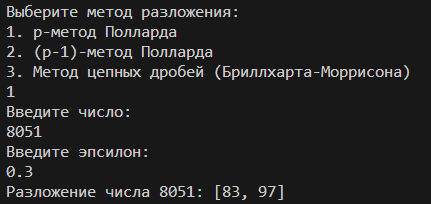
\includegraphics[width=0.8\textwidth]{pic/1.png}
        %     \caption{Тест первого алгоритма факторизации чисел}
        % \end{figure}

        % \begin{figure}[H]
        %     \centering
        %     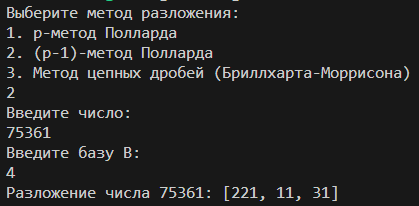
\includegraphics[width=0.8\textwidth]{pic/2.png}
        %     \caption{Тест второго алгоритма факторизации чисел}
        % \end{figure}

        % \begin{figure}[H]
        %     \centering
        %     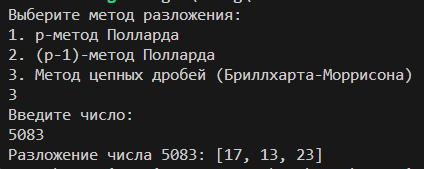
\includegraphics[width=0.8\textwidth]{pic/3.png}
        %     \caption{Тест третьего алгоритма факторизации чисел}
        % \end{figure}

\conclusion

    В данной лабораторной работе были изучены теоретические сведения о методах
    дискретного логарифмирования (метод Гельфонда-Шенкса, $\rho$-метод Полларда,
    метод вычисления дискретного логарифма в конечных полях). На их основе были
    рассмотрены соответствующие алгоритмы. Была произведена оценка сложности
    созданных алгоритмов. Они послужили фундаментом для программной реализации,
    которая впоследствии успешно прошла тестирование, результаты которого были
    прикреплены к отчету вместе с листингом программы, написанной на языке Rust
    с использованием стандартных библиотек языка.

\end{document}
